\documentclass{article} % For LaTeX2e

\usepackage{nips14submit_e,times}
\usepackage{hyperref}
\usepackage{url}
\usepackage{graphicx}

\usepackage{listings}
\usepackage{color}

\definecolor{lightgray}{rgb}{1,1,1}
\definecolor{darkgray}{rgb}{.4,.4,.4}
\definecolor{redstrings}{rgb}{0.64,0.08,0.08}
\definecolor{blue}{rgb}{0,0,1}
\definecolor{greencomments}{rgb}{0,0.5,0}
\definecolor{cyan}{rgb}{0.0,0.6,0.6}

\renewcommand{\lstlistingname}{Code fragment}


\lstdefinelanguage{JavaScript}{
  keywords={break, case, catch, continue, debugger, default, delete, do, else, finally, for, function, if, in, instanceof, new, return, switch, this, throw, try, typeof, var, void, while, with, null},
  keywordstyle=\color{blue}\bfseries,
  ndkeywords={class, export, boolean, throw, implements, import, this},
  ndkeywordstyle=\color{blue}\bfseries,
  identifierstyle=\color{black},
  sensitive=false,
  comment=[l]{//},
  morecomment=[s]{/*}{*/},
  commentstyle=\color{greencomments}\ttfamily,
  stringstyle=\color{redstrings}\ttfamily,
  morestring=[b]',
  morestring=[b]"
}

\lstset{
   language=JavaScript,
   backgroundcolor=\color{lightgray},
   extendedchars=true,
   basicstyle=\footnotesize\ttfamily,
   showstringspaces=false,
   showspaces=false,
   numbers=left,
   numberstyle=\footnotesize,
   numbersep=9pt,
   tabsize=2,
   breaklines=true,
   showtabs=false,
   captionpos=b
}


%\documentstyle[nips14submit_09,times,art10]{article} % For LaTeX 2.09


\title{Inspecting community evolution using text and network structure}


\author{
Mario Karlovcec, Jan Rupnik, Primoz Skraba \\
Artificial Intelligence Laboratory\\
Jožef Stefan Institute\\
Jamova cesta 39, Ljubljana, Slovenia \\
}

% The \author macro works with any number of authors. There are two commands
% used to separate the names and addresses of multiple authors: \And and \AND.
%
% Using \And between authors leaves it to \LaTeX{} to determine where to break
% the lines. Using \AND forces a linebreak at that point. So, if \LaTeX{}
% puts 3 of 4 authors names on the first line, and the last on the second
% line, try using \AND instead of \And before the third author name.

\newcommand{\fix}{\marginpar{FIX}}
\newcommand{\new}{\marginpar{NEW}}

% \nipsfinalcopy % Uncomment for camera-ready version

\begin{document}


\maketitle

\begin{abstract}
Detect communities in several timestamps, connect them in neighbouring timestamps, extract keywords in communities and analyse structure and topic change.
\end{abstract}

\section{Introduction}

In this work we propose an approach for detecting, visualizing and modelling community evolution of dynamic networks using textual features and graph structure. The approach is implemented in QMiner – open source data analytics platform for processing streams of structured and unstructured data \footnote{http://qminer.ijs.si/}. QMiner integrates machine learning algorithms with network analysis based on SNAP library \cite{snap}.

Mapping between communities and clusters.

Building community evolution model.

Predict splits and merges.

Examine homophony and heterogeneity.

Use hub nodes (page rank, centrality, etc.) members to track communities/clusters.

K-means clustering (e.g. num. of communities in t for K)

Keywords extraction for community description

Communities are often defined using the network topology as groups of nodes with many links inside the groups but a few links between them . Finding communities is looking for a partition of the nodes that maximizes a quality function which captures the idea of dense groups communities \cite{aynaud}. One such broadly used quality function is modularity \cite{newman2003}.

\section{Related work}

Standard methods for studying communities in evolving networks usually fall into three groups: (1) Static algorithms which study snapshots independently  and connect the resulting communities, (2) using temporal information directly in community detection methods and (3) using incremental/online algorithms \cite{aynaud}. In this work, we apply the first approach of independently computing communities, following by solving community matching/tracking problem to obtain the community evolution. The benefit of  the static approach is that in this context, the problemh as been  well-studied, with many different algorithms developed (see Clauset-Newman-Moore\cite{clauset-newman-moore}, ...). The main drawback is  instability \cite{aynaud2010}. When the underlying algorithms are  non-deterministic, a small modification of the input network may lead to large changes in the resulting community partition.
 
Identifying the relationships between the neighbouring partitions is often referred to as the matching or tracking problem. It is a crucial step in using static algorithms on dynamic networks as it help us identify patterns in the communities. One approach, 
MONIC \cite{spiliopoulou}, is a general methodology for modelling and tracking external and internal cluster transitions, that include: survival, split into multiple clusters, absorption, disappearing and emergence of a new cluster. In line with the set-theoretic approach of  the MONIC methodology, in \cite{gliwa2013} authors determine the  matching of clusters by calculating a modified Jaccard coefficient, with an additional constraint on difference in cluster sizes. Other approaches of solving the matching problem include using key nodes in the clusters \cite{wang} and community detection algorithms for the matching problem\cite{palla}.

Topic evolution graph to trace topic transitions \cite{mei2005}.
Predicting community evolution problem is tackled in \cite{gliwa2013}. Predictions are based on the previous events in group lifetime described by group size, cohesion, leadership and density.

\section{Approach}
Our approach is generic,  given a dynamic graph, each snapshot is analyzed using any statistical community detection algorithm. The detected communities are then matched and a directed graph representing community evolution is constructed. In our context, the input graph has text associated with each node. We extract keywords from the text 
 to describe the content of the communities. Finally, community evolution is visualized as a directed graph, using different colours and sizes of nodes and arcs.  Based on the extracted keywords and the graph structure, a rich feature set is constructed. We test the feature set by using it to construct a classification model for the communities.  

\begin{figure}\label{architecture}
   	\begin{center}
   	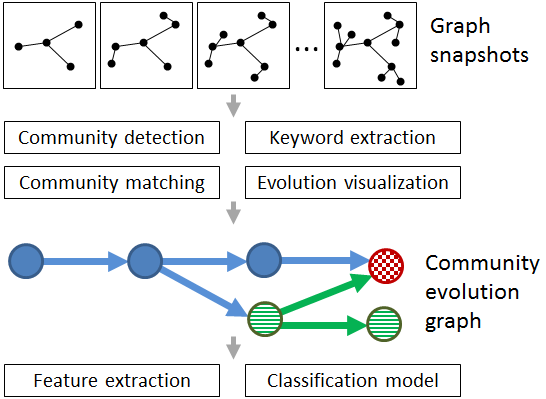
\includegraphics[width=0.6\textwidth]{architecture.png}
   	\end{center}
   	\caption{Approach}
\end{figure}
\subsection{Community detection and matching}
The input for the proposed approach is a set of snapshots of an evolving graph. A statistical community detection algorithm is applied on each snapshot. The types of supported input snapshot graphs depends on the specific community detection algorithm. These may be  undirected or directed, weighed or unweighed graphs. The approach is independent of the choice of the community detection algorithm, making it modular and applicable on the wide range of different algorithms. In our experiments we use Clauset-Newman-Moore\cite{clauset-newman-moore} algorithm. Communities as groups of members obtained from each snapshot serves as input for the community matching. The community matching problem can be reduced to determining whether a community in time $t$ exists in time $t+1$ and to which community it maps to if it exists. This is determined by calculating a modified Jaccard measure (similar as in \cite{gliwa2013})  between each pair of neighbouring communities. Let  $A$ be a community at $t$ of size $|A|$ and $B$ a community at $t+1$ of size $|B|$. The similarity measure is:
\begin{equation}
\alpha = \frac{A\cap B}{|A|},
\beta = \frac{A\cap B}{|B|}.
\end{equation}
If there are a pair of communities $A$ and $B$ such that $alpha > \tau_{alpha}$ and $beta > \tau_{beta}$, where are $\tau_{alpha}$ and $\tau_{beta}$ are two thresholds restricted to the interval $(0.5, 1]$, we say community $B$ represents the continuation of $A$ at $t+1$. Otherwise, if there is no match, community $A$ decays at $t$ and $B$ represents a new community emerged at $t+1$. Thresholds closer to 1 set stricter conditions for maintaining a cluster in the future time point. Higher value of $\tau_{alpha}$ increases the required proportion of elements in $A$ that must be retained in the same community in the future time point. $\tau_{beta}$ threshold sets the 'purity' requirement, i.e the minimum proportion of elements in B that come from A. In case $\tau_{beta} = 1$, no new elements, or those from other communities than $A$ are allowed in $B$ in order to match $A$ with $B$. Restricting both thresholds to the interval $(0.5, 1]$, we ensure that each community can be matched with at most one community in the future time point. Since stability of communities can pose a difficulty in our approach, we choose $\tau_{alpha} = \tau_{alpha} = 0.5$ for the initial settings, but also experiment with other threshold values.

\subsection{Keyword extraction}
Keyword extraction process is done by first uniting textual descriptions of nodes of a community into documents. Since the members of the communities change over time, a separate document is generated for each occurrence of a community.The next step is to create bag-of-words feature space representation of the collection of documents, where each document is a vector of n-grams. Bag-of-words representations of documents are created by the standard approach involving tokenization, stop-words removal, stemming using English Porter stemmer, tf-idf weighting and normalization. The final step of the keyword extraction process is to select a number of n-grams with highest tf-idf scores from each documents.  In our experiments, we usually choose 10, since we found this is sufficient for interpreting communities. These n-grams are the keywords that represent the content of communities.

\subsection{Visualization}
An important part of this work is visualization of the community evolution. This enables quick inspection of  interesting events in graph evolution, such as sudden splits and merges of communities. For example, a community with stable evolution with few communities and rear splits and merges, may at some point explode with many splits and the emergence of new communities. Such  an atypical change in the structure  could easily be identified with our  visualization. The evolution of communities is visualized as a directed graph, with nodes representing communities and arcs showing the relationships between communities in consecutive time points. Arcs are drawn whenever two neighbouring communities share common members. The size of the nodes corresponds to the number of member of communities, while width of the arcs fits the number of shared members and is relative to the diameter of the nodes. Colour is used to indicate whether two connected neighbouring nodes represent the same community. The extracted keywords are assigned to the nodes in the directed graph, improve the interpretation of the evolution by giving context and information on the content of communities.
 
\subsection{Feature extraction}
When building our community evolution model, we use features extracted from the text assigned to communities, as well as features based on  the graph structure. The text-based features are constructed by performing text-based clustering of the community members for each time $t$ and mapping between communities and clusters. At each time,  all the members of a  community are represented using the bag-of-words feature vector representation. This process is similar to keywords extraction step, but rather than grouping the members by community, each member is represented as a separate BOW vector.  We then cluster the members based on text. If the clustering method requires a parameter for specifying the number of clusters (e.g. K-means), the number of communities at time point $t$ is used. After clustering, mapping between each community and cluster is performed. Each community gets a vector with number of elements corresponding to the number of clusters it maps to. The values of the vector are proportions of elements from a community mapped to a cluster. This vector is the basis for deriving two features: (1) {\bf the number of significant clusters it maps to} and (2) { \bf the uniformity of the mapping}.

The first feature counts the number of mappings greater than a threshold restricted to the interval $[0, 1]$. In the experiments we used $K^{-1}$, where K is  the number of communities at time point $t$. The second feature, uniformity of the mapping distribution is computed  using Shannon's entropy formula.

The graph structure based features we use are: centralization \cite{freeman1978}, density\cite{wasserman1994}, cohesion and group size.

\section{Experimental results}
Build community evolution model.
Use the model for prediction on different datasets (co-authoring, companies, ...). Evaluation

\begin{table}[t]
\caption{Sample table title}
\label{sample-table}
\begin{center}
\begin{tabular}{ll}
\multicolumn{1}{c}{\bf Dataset}  &\multicolumn{1}{c}{\bf DESCRIPTION}
\\ \hline \\
Dendrite         &Input terminal \\
Axon             &Output terminal \\
Soma             &Cell body (contains cell nucleus) \\
\end{tabular}
\end{center}
\end{table}

\section{Conclusion and discussion}

\subsubsection*{Acknowledgments}
   The authors gratefully acknowledge that the funding for this work was provided by the project X-LIKE (ICT-257790-STREP)\cite{xlike}.


\bibliographystyle{unsrt}
\bibliography{communities}

\end{document}